\documentclass[10pt,letterpaper]{report}
%\usepackage[utf8]{inputenc}
\usepackage{amsmath}
\usepackage{amsfonts}
\usepackage{amssymb}
\usepackage{graphicx}


%\usepackage[T1]{fontenc}
%\usepackage[urw-garamond]{mathdesign}
\usepackage{venturis2}

\author{Andrew Rosen}
\title{Attributes of Distributed Hash Tables and Their Ramifications}
\begin{document}
\maketitle
\setcounter{tocdepth}{4}



\tableofcontents

\chapter{Introduction}
Let's begin with a discussion of definitions:  what is a Distributed Hash Table?
A Distributed Hash Table, or DHT, is a data structure with the key-value mapping capabilities of a Hash Table, but the contents of the table is distributed among nodes in a network.
Each node stores a subset of the entire lookup table and a subset of all the stored values.
One node in DHT a can find the node responsible for any particular key-value pair without any single node knowing all the routing information for the network\footnote{Two exceptions here.  
The first is in a sufficiently small network, nodes will naturally know  all node in the network. This scenario can largely be ignored.  The second case is ZHT, which assumes a network with very specific conditions.}




Structured P2P systems and DHTs are so closely related that they often are talked about interchangeably  \cite{wu2004handbook} \cite{lua2005survey}. 


\section{History}

Flooding is not scalable \cite{can} (which cited something else).


\subsection{Why DHTs}
\cite{malkhi2001viceroy} -  Between congestion, cost of join/leaves, and lookup time there are tradeoffs.  
Optimizing for two can be done but has bad cost.
For example, a balanced binary tree has congestion at root.


\section{The Coordinate System, Responsibility and Neighbors}


There are two  broad types of objects that exist in a DHT: Nodes and data.  
Nodes are the actual members of the DHT; they store a portion of the lookup table and a subset of the data they are responsible for. 
% \cite{dolr} defines as ``A node represents an instance of a participant in the overlay''
For clarity, I will call the keys mapped to nodes \textit{ID}s. 

All DHTs assign responsibility the same way:  the node with an ID that is ``closest'' to a particular key is responsible for that key.  
However, the definition of ``closest'' differs from protocol to protocol.
One metric used by Chord (others) is "the node with the closest id larger than the key" (presumably, this is much easier to code than ``the closest without going over.'').


Almost every DHT operates in a modulus space.  The space can be either bidirectional (symphony) or unidirectional (Chord).
The overlay shape/layout is actually as important as the peer list or routing algorithm.
There's typically a distance function, but it's not very interesting.

The vast majority of overlays only use a single coordinate (and therefore a single dimension).  
This coordinate is assigned essentially at random through a hash function, .  
If more than one dimension is used, coordinates can be chosen to map to a particular physical feature (geographical location  or available bandwidth) or a metric (trust or influence).

\subsubsection{The Keyspace}
The keyspace is the domain of keys that can be assigned to nodes and data using the  consistent hashing algorithm.  

The domain of the keyspace can be $m$-bit identifiers, or floats from 0-1.  So long as $m$ is the same it is possible to map from one to another.

\subsection{Hashing Algorithms}
SHA1, LSH

Hash Collisions are ignored since the size is so large.
Consistent Hashing is a must.

\subsubsection{Landmark Based}
Ratnasamy et al. \cite{can} present the concept own using landmarks to choose coordinates, rather than a has function.
Each node measures the round-trip time (RTT) to each to of the $m$ landmarks, which yields one of $m!$ permutations.
The keyspace is partitioned into $m!$ regions, each corresponding to one of the orderings.  
A joining node now chooses a random location from the region corresponding to its landmark ordering.

This scheme greatly decreases stretch, but at the cost of losing the random and uniform distributed provided by hash functions.  
Fault tolerance in the network is compromised, since geographically close nodes will be assigned close locations. 
An event that disables a large geographic region can now disable the entire network, since the damage will affect an entire region, rather than being spread throughout the network.

\subsection{Closest Metrics}

The advantage of using a successor or predecessor metric that changes in responsibility due to node failure are recognized immediately.  
In a literal ``closest to the key'' metric, there is computation involved. The closest node can be referred to as the 

\begin{itemize}
	\item The responsible node.
	\item Predecessor/Successor \cite{chord}
	\item The \textit{root} node or just the \textit{root} \cite{tapestry}.

\end{itemize}

\subsubsection{Literal}
As in literally the closest.  The cost is computation, but the benefit is that the metric is natural and easy to understand

\subsubsection{Successors}
This is the way Chord works;  from the node's perspective, a node is responsible for the keys between its ID and that of its predecessor.   Fault tolerance

\subsubsection{Predecessors}
This is the opposite of how the successor scheme works and interestingly enough, easier to describe.  The node with the ID closest without going over a key is responsible for that key.  Fault tolerance here works identically to the successor scheme, just in the other direction.


\subsubsection{Groups}

See Pastry

\subsubsection{Regions}
In a Voronoi or georgraphic based hashing environment, a node's responsibility would be defined by a region of some kind





\section{The Peerlist}


\subsection{Creating the Peerlist}
We can (can we?) break this down in a couple of ways.  Gossip vs nongossip (security)


Some DHTs build their peer lists by using suggestions from other nodes.  The issue with this is that this opens up a new vector for attacks.   A malicious node can lie to another node about what peers to use, but even worse, these lies can then propagate to other nodes.

Others DHTs choose their peers by finding the node closest to a particular ID.  For example, a node in Chord chooses fingers by finding the node closest to its ID plus some  power of 2.    In Symphony, peers are chosen by finding the node closest to some ID, chosen randomly over a probability distribution.



\section{The Lookup Operation} 

Lookup and Routing are synonymous

All routing algorithms follow the same scheme:  the next hop  brings me closest to my destination.  The very nature of DHTs makes the routing process greedy, and the node chooses the best path based on its peer list (It is possible to use a 1-ahead lookup, thereby keeping a record of your peer's peerlist.  The cost becomes quite large for more than two, but routing does speed up.).  Specifics aside, there are two ways to look at routing.  The first way  answers the question ``Who is responsible for this particular key?''  but rather than asking the entire network, it assumes the entire network consists only of it and the peer list.  The other way to look at it that routing is the process of greedily  eliminating possible recipients, until the final node must be the node responsible.  

Almost every DHT has a $lg(n)$ routing time, eliminating  half of the remaining nodes each step.
However, Kleinberg Small World Networks have inspired networks that have a polylogarithmic time in exchange for smaller peerlists and routing tables.



\subsection{Who Decides The Search Stops}
Iterative vs Recursive

Should the owner decide?  Should it predecessor?

\subsection{Lookup Time vs Table size}

Average lookup times and average degrees are not useful metric:
Contrived hypersphere has constant lookup time and avg constant degree,



Actual worst, actual best, and the distribution between them.  Expected worst case is important to analyze.

\subsection{Bidirectional links don't matter except when they do.}

\section{Churn and Fault Tolerance}  % not nessuicarily the same, ie what happens when we route wrong

DHTs can choose various ways to implement fault tolerance.  First, a DHT must have some mechanism for neighbors to take over for node failure (although it doesn't have to).  Next is peerlist maintenance.  How are failed lookups handled?  How do you handle churn?


Reactive vs periodic


\subsection{Design Considerations of Churn}

Any comparison of DHTs have to be done with respect to churn.    Any analysis  that focuses on a unchanging network is sorely lacking (unless the DHT is designed to work solely in an essentially static network. \cite{lichurn}  evaluates DHTs in terms of cost vs performance, cost being the cost of keeping the routing tables up to date and performance being latency, not hop count.  \cite{lichurn} examined Tapestry, Chord, Kademlia, and Kelips and simulated a size 1024 network in a $2^64$ keyspace.   

They found no optimal configuration of DHT settings, but for a given cost, there is an optimal latency, and vice-versa.  This is represented by convex hulls on a graph (Chord had the best looking convex hull, but it should be noted among the authors are people involved in Chord).   The authors tested each parameter to find the effect each had on the cost/performance ratio.

Chord was found to use bandwidth efficiently due to stabilizing successors/neighbors rather than peers/fingers  (this is good behavior for the simulation, as this means while there may be more hops, there won't be penalty from trying to talk to a dead node).  In other words, because Chord has two maintenance procedures, one that makes sure the network remains healthy and the other that periodically makes sure shortcuts are properly spaced, the network maintains a high level of correctness, compared to the other three.

Increasing the number of parallel lookups from Kademlia decreased the latency, but increased traffic.  Increasing the maintenance rate in Kademlia increased the traffic but produced no noticeable improvement on lookup time.  This is because more dead entries are cleaned from the routing table, but the parallel lookup prevented bad entries from having a detrimental impact in the first place.  "Base" was not varied in Kademlia.

Chord modifications:  

Responsibility falls to the predecessor rather than successor.   (uninteresting)
When looking for a node to put in finger f, Chord first finds the node appropriate for that entry, then pings it and it's successors.  The fastest node is put into that finger.  (interesting)
There is a ``base'' parameter, which is different than the base used to describe the size of the keyspace;  a base of $b$ means each node  holds $(b-1)(log_b n)$ fingers.  The network being tested is size 1024, but in a $2^64$ keyspace;  Chord would typically use 64 fingers.   Unsurprisingly and not discussed, as $(b-1)(log_b n)$ approaches 64, the shape of the convex hull improves and slowly degrades as $b$ increases, as unnecessary cost is introduced  (uninteresting but necessary for the paper's conclusion).


\subsection{Failure Detection}
DHTs can have different methods of detecting failure.
The consequences of this are largely unexplored.
Perhaps check churn convex hulls.
\begin{itemize}
	\item Heartbeat based scheme involve nodes periodically broadcasting their existence to their neighbors, possibly with other data.  A failure is detected when a node fails to hear from the neighbor after a certain number of cycles.  CAN uses this.
	\item Checking schemes involve a node periodically checking its neighbors, querying them to see if they're alive.  This can be combined with maintenence operations to adjust the routing tables of nodes.
	\item Reactive detect only when a query fails
\end{itemize}

\subsection{Induced Churn}

Other authors have examined using manually causing  churn to help with network performance.
Inducing churn keeps the network in continuous flux, making it hard to keep tables poisoned.   
This isn't a good idea where data needs to be stored, but for anything else, like query processing and monitoring, there's considerable benefits. 

The motivation of this paper was to create a  defense against route poisoning that didn't rely on a trusted central authority and create a defense against eclipse attacks that helped boost performance.  
It expands on the idea of keeping two routing tables, one that is optimized for speed, the other for robustness and security.

The goal is to keep the average level of table poisoning down.  
Rather than using the secure table as a fallback, the optimized table is always used, but periodically resets to the secure table.  
Optimizing the table then starts again.

Furthermore, nodes choose a new ID periodically, thus making the network more unpredictable to the attacker.  
The authors suggest adding a deterministic nocne to the ip/port hashing (and they seem to describe the measure that Brendan described to to predict where a node is, but there's no use of public keys, as far as I can tell)

Their implementation is called maewlstrom, and it is built on top of the Bamboo DHT.



\section{Geometry}


\section{Security}

I believe there are two very broad categories for thwarting adversaries:  a)  preventing malicious nodes from joining the DHT b) preventing what malicious nodes can do when they have joined the DHT.  The two are intractably mixed.  In the vast majority of cases, there is no way to prevent all possible malicious nodes from joining, so steps must be taken to mitigate the actions of malicious nodes in the network so that a single node or fraction of nodes cannot destroy the network.  On the flip side, no matter what limits you place on individual nodes, if attacker can become the majority/plurality of the network, he gets to do whatever he wants.

The problem of detection might be considered a third category;  after all, once you detect a malicious node or attempt to join, you can act on that information (hopefully).

All of the below is from the following survey \cite{dhtsec}


So first off, what are general statements that are true about all DHTs?
DHTs  effectively act as a decentralized lookup service.  Or a routing service.  It really depends.  But in essence each member is assigned a key, used as an identifier and for determining responsibility.
DHTs can be quite large.
DHTs have to load balance.
Each node will (probably) only know a small subset of nodes in the network.
DHTs have to deal with churn (flash crowds too but that's solved by IRM and other replication techniques)
\cite{dhtsec} says any distributed system is vulnerable to DDOS and exploits specific to a particular implementation (duh), but in particular note these two closely related exploits. 

Sybil (creating malicious nodes)
Eclipse (isolating real peers)

There is close overlap between these two (a large enough Sybil attack become an Eclipse attack) and both attacks are just about establishing control of the network so an actual attack can be carried out.




\subsection{Sybil Attacks}
The Sybil attack is basically one of ChordReduce's advantages, but turned up to eleven to be made into an attack.  So, in ChordReduce, we said that basically if we wanted a node to do more work,  it creates another instance of the program on a different port.  Since we hashed the IP address and the port to get the ID of the node, we could create an arbitrary number of extra nodes!  Now imagine you're an attack and you know that...

The Sybil attack was defined in 2002.  Basically,  if there's no way to guarantee that a single node in the network is a one-to-one mapping to some device in the outside world, we can just create as many nodes as we want with a single device.  A DHT can operate when a small fraction of the nodes in the network are malicious, but this is a bit more than a small fraction.  

Named after poor Sybil, a case of dissociative identity.

\subsubsection{What Can the Sybil Attack Do}
Once a Sybil attack has been launched,  the adversary effectively controls the network.   He could insert false records into routing table of legitimate nodes.  I could just drop all traffic routed to me.

\subsubsection{Prevention}


Sybil attacks can be prevented by ensuring each node represents only a single physical entity (this naturally can limit some load-balancing capabilities of the DHT). There's several categories for Sybil defences proposed by \cite{dhtsec}.  I'll list I found pertinent.

The first and allegedly most successful is a centralized authority.  Castro et al says the only way is to exclusively generate node IDs using a trusted CA (hey, didn't we propose a distributed trusted CA using a blockchain?).   Certificates bind public key and ip to an ID. This doesn't work from some DHTs.  If nodes and responsibility are defined by a coordinate, then it works great.  If responsibility is defined by a space (say like a Voronoi region), then it's not so great.  \cite{dhtsec} states that certificates are the best defence, but then it becomes a question of preventing the adversary from gaining legitimate certificates.  The best solutions they could come up with for that are a) charge money b) map meatspace ids to to node ids in a preexisting network.  The big problem from our point of view is a centralized resource is single point of failure/obvious target.   Take the CA down, and the network will fall apart/nodes can't join.  Or even worse, an adversary could be your CA ("When confronted with an impregnable fortress, well-garrisoned and well-stocked with provisions - endeavour to be the man on the inside." - Terry pratchett).

The obvious step after that is a decentralized registration approach. This has issues stemming from the limited view of the network and knowing who to trust.  (this is a problem we can solve/ improve upon)

A couple of schemes have been suggested to do away with hashing  IP addresses for IDs and instead  look at using router ip address and mac addresses.   The original Pastry paper (before the Sybil was defined) mentioned possibly using the hash of a public key.

A couple of authors suggest incorporating puzzles: Borisov et al and Rowaihy et al.  Borosov suggested that nodes need to solve hash values during the ping period.  Obviously not so hard for a single node, but it prevents the number of nodes a single computer can impersonate.  Rowaihy suggested a hierarchical tree structure with a root and a few trusted members. Prospective nodes solve hashes for leaf nodes and work their way up the parents, solving more puzzles, until authenticated by the root.   (but depending on the difficulty  and the hash algorithm involved, this might be defunct because of Bitcoin.  There's cheap and powerful ASICS for SHA right now.  Solving for hash values always makes me think of Bitcoin mining)



\subsection{Eclipse Attacks}
The Eclipse attack is very much related to the Sybil attack.  The goal of Eclipse attack is to infect the peer lists (fingers) of a sufficient fraction of nodes, such that the vast majority of messages will be routed to malicious nodes.  Naturally  a large enough Sybil attack is  going to cause an Eclipse attack. \cite{dhtsec} states that networks with well defined rules for joining peers, such as Chord, are naturally immune to Eclipse attacks, although well defined is not... well, well-defined in the paper.  Based on the reading I have done, I take it to mean that because Chord doesn't construct its finger table from info provided by other nodes in a broadcast, but from network queries .  Although it was not examined, due to Symphony's nature of choosing  fingers using a random distribution, it should be immune in the same manner.

An Eclipse attack begins with a compromised or malicious node (we'll just use malicious) \cite{induced}.  In an open system, like the vast majority of use cases for DHTs, it is very reasonable to assume this can occur.  Malicious nodes can only affect messages that are sent or forwarded to them, so the adversaries  goal is (re)direct the majority of the overlay's traffic to malicious nodes, preventing the normal/good nodes from communicating without routing through a malicious node.   Thus, the malicious nodes eclipse the good nodes.

The redirection can be done in a few ways.  First and most blunt is via a Sybil attack.  If the adversary creates enough virtual nodes, the majority of the network traffic will have to be directed to malicious nodes.  This attack works wherever a Sybil attack works  (Note: this may be a potential  misclassification on my part; I have to see how more papers treat the difference between Sybils and Eclipse.).

The second type of attack exploits the routing table maintenance of DHTs that use a "gossip"- based approach.  The malicious nodes exploit the peer selection process and poison the routing tables of good nodes so that traffic will be routed to malicious nodes.  This could be done by falsely responding to queries or by spoofing messages and impersonating other nides.   Depending the specifics of  the maintenance and discovery procedures,  the process could cascade with nodes unwittingly poisoning one another.

One possible way:  Most DHTs store node information in a tuple: (ID, ip, port).  An attack simply feeds nodes fake IDs ( chosen either statistically or in response to a request) with a malicious node's ip:port.  If node ID is generated via hash(ip,port)  this can be mitigated someone by verification  




\chapter{The Essential DHTs}% Structured Overlays for Distributed Hash Tables

\subsection*{Shared Attributes}
% log routing log table

\begin{itemize}
	\item \textbf{Stretch} \cite{hildrum2004distributed} - The ratio of distance traveled by the lookup compared to the actual lookup distance. Our VHash experiments were some about determining that VHash had a lower stretch that Chord.
	\item $n$ will always refer to the network size.
	\item $N$ should be used to explicitly refer to the Namespace/keyspace size.
	\item Lookup $\equiv $ Routing
	\item Attacks only focus on attacking the base implementation. 
	\item Geometry and organization of the network as a whole is a function of the peerlist.
	

\end{itemize}











\section{Chord}
Chord \cite{chord} is a peer-to-peer (P2P) protocol for file sharing and distributed storage that guarantees a high probability $\log_{2} N$ lookup time for a particular node or file in the network. 
It is highly fault-tolerant to node failures and churn, the constant joining and leaving of nodes.  It scales extremely well and the network requires little maintenance to handle individual nodes.  
Files in the network are distributed evenly among its members.

As a distributed hash table (DHT), each member of the network and the data stored on the network is mapped to a unique $m$-bit key or ID, corresponding to one of  $2^m$ locations on a ring. 
The ID of a node and the node itself are referred to interchangeably.

In a traditional Chord network, all messages travel in one direction - upstream, hopping from one node to another with a greater ID until it wraps around.
A node in the network is responsible for all the data with keys \textit{above or upstream} his predecessor, up through and including its own ID.  If a node is responsible for some key, it is referred to being the successor of that key.

Robustness in the network is accomplished by having nodes backup their contents to their $s$ (often 1) immediate successors, the closest nodes upstream.  
This is done because when a node leaves the or fail, the most immediate successor would be responsible for the content its content.

Each node maintains a table of $m$ shortcuts to other peers, called the finger table.   The $i$th entry of a node $n$'s finger table corresponds to the node that is the successor of the key $n+2^{i-1} \mod 2^m $.  Nodes route messages to the finger that is closest to the sought key without going past it, until it is received by the responsible node.  This provides Chord with a highly scalable $\log_2(N)$ lookup time for any key \cite{chord}.

As nodes enter and leave the ring, the nodes use their maintenance procedures to guide them into the right place and repair any links with failed nodes.  Full details on Chord's maintenance cycle are beyond the scope of this paper and can be found here \cite{chord}.


\section{CAN}
Unlike the other DHT presented in this chapter, the Content Addressable Network (CAN) \cite{can} works in a $d$-dimensional torus, with the entire coordinate space divided among members.
A node is responsible for the key-value pairs that fall within the ``zone'' it owns.
Each key is hashed into some point in the coordinate system.

\subsection*{Peerlist and Geometry}
CAN uses an exceptionally simple routing table.  
Every node in the CAN network is assigned a geometric region in the coordinate space and each node maintains a routing table consisting each node that borders the node's region.

The size of the routing table is a function of the number of dimensions $O(d)$. 
The lower bound on the routing tables size in a populated network (eg, a network with at least $2d$ nodes) is $\Omega(2d)$.  
This follows that along each axis, there is at least one node bordering the zone along each end of the axis.
The size of the routing table can grow as more nodes join and the space gets further divided; however, \textbf{•}algorithms prevent the regions from becoming too fragmented.



\subsection*{Lookup}
As previously mentioned, each node maintains a routing table corresponding to their neighbors, those nodes it shares a face with.
Each hop forwards the lookup to the neighbor closest to the destination, until it comes to the responsible node.
In a space that is evenly divided among $n$ nodes, this simple routing scheme uses only $2 \cdot d$ space while giving average path length of $\frac{d}{4}\cdot n^{\frac{1}{d}}$
The overall lookup time of in CAN is bounded by $O(n^{\frac{1}{d}})$ hops\footnote{Around the same time CAN was being developed, Kleinberg was doing research into small world networks \cite{kleinberg2000small}.  He proved similar properties for lattice networks with a single shortcut.  What makes this network remarkable is lack of shortcuts.}.

% fault tolerence in routing
If a node encounters a failure during lookup, the node simply chooses the next best path.
However, if lookups occur before a node can recover from damage inflicted by churn, it is possible for the greedy lookup to fail.
The fallback method is to use an expanding ring search until a candidate is found, which recommences greedy forwarding.

\subsection*{Joining}
Joining works by splitting the coordinate space.  
If node $n$ with location $P$ wishes to join the network, it contacts a member of the node to find the node $m$ currently responsible for location $P$.
Node $n$ informs $m$ that it is joining and they divide $m$'s region such that each becomes responsible for half.


Once the new zones have been defined, $n$ and $m$ create its routing table from $m$ and its former neighbors.
These nodes are then informed of the changes that just occurred and update their tables.
As a result, the join operation affects only $O(d)$ nodes.  



\subsection*{Repairing}

Churn that occurs with warning has almost no effect on the network.
A leaving node, $f$, simply hands over its zone to one of its neighbors of the same size, which merges the two zones together.
The complications occur if this is not possible, in which case  $f$ hands the zone to its smallest neighbor, who must wait for this fragmentation to be fixed.

Unplanned failures are also relatively simple to deal with.
%failure detection is heartbeat based
Each node broadcasts a heartbeat to its neighbors, containing its and its neighbors' coordinates.
If a node fails to hear a heartbeat from $f$ after a number of cycles, it assumes $f$ must have failed and begins a \texttt{takeover} countdown.
When this countdown ends, the node broadcasts\footnote{This message is sent to all of $f$'s neighbors;  I assume that nodes must keep track of their neighbors' neighbors.} a \texttt{takeover} message in an attempt to claim $f$'s space.
This message contains the node's volume.
When a node receives a \texttt{takeover} message, it either cancels the countdown or, if the node's zone is smaller than the broadcaster's, responds with its own \texttt{takeover}.

The general rule of thumb for node failures in CAN is that the neighbor with the smallest zone takes over the zone of the failed node.
This rule leads to quick recoveries that affect only $O(d)$ nodes, but requires  a zone reassignment algorithm to remove the fragmentation that occurs from \texttt{takeovers}.

As mentioned earlier in the text, Ratnasamy et al. \cite{can}  also present the concept own using landmarks to choose coordinates, rather than a has function.
Each node measures the round-trip time (RTT) to each to of the $m$ landmarks, which yields one of $m!$ permutations.
The keyspace is partitioned into $m!$ regions, each corresponding to one of the orderings.  
A joining node now chooses a random location from the region corresponding to its landmark ordering.

\subsection*{Attacks}








\subsection*{Design Improvements}
Ratnasamy et al.\ identified a number of improvements that could be made to CAN \cite{can}.
Some of these improvements have already be explored in Chapter 1.

One modification to the system is increasing the number of dimensions in the coordinate space.
Increasing $d$ improves fault tolerance and reduces path length.

One concept Ratnasamy et al.\  introduces is the idea of multiple coordinate spaces existing simultaneously, called \textit{realities}. 
Each object in the DHT exists at a different set of coordinates for each reality simultaneously.
So a node might have coordinates $(x_0,y_0,z_0)$ in one reality, while having coordinates $(x_1,y_1,z_1)$ in another.
Independent sets of neighbors for each reality yield different the overall topologies and mappings of keys to nodes.
Multiple realities increase the cost of maintenance and routing table sizes, but provide greater fault tolerance and greater data availability.
 
A final  modification is to allow multiple nodes shares the same zone (ie zones don't necessarily split as a result of a join operation).    
\section{Pastry}

Addressing - 128 bit ID, 0 to $2^128 -1$, assigned randomly using hash.   but thought of as base $2^b$ numbers (typically b=4).  This creates a hypercube topology \cite{induced}.

\subsection*{Peerlist}
Pastry's peerlist consists of three components: the routing table, a neighborhood set and a leaf set.  The Routing table consists of $\log(n)$ rows and $b$ columns each. Each  
The 0th row contains peers which don't share a common prefix.  The 1st row contains those that share a length 1 common prefix, the 2nd a length 2 common prefix, etc.  Since each ID is a base $2^b$ number, there is one column for each possible difference.   The i,j entry of the table contains an ID that shares the same first i digits, with digit i+1 having a value of j (yes, a slot is wasted in each row).

The neighborhood set hold the ID and Ip address of the closest nodes, defined by a metric.  It is not used for routing.  The leaf set is used to hold the numerically closest nodes. Half of it for smaller and half for larger.


\subsection*{Lookup}
Forwarded to (node/peer?) whose shared prefix is longer.  If no one  has a better shared prefix than the current node, the message is forwarded to the closest  node.




\subsection*{Joining}
The table is populated at first by a join message to the node responsible for the joining node ID.  
As part of the join message, nodes  along the path send their routing tables.  
After the joining node creates it's routing table, it sends a copy to each node in the table, who then can update their routing tables.   
Node join cost is $O(log_2^b n)$ messages  with  a constant  coefficient  of $3*2^b$




\subsection*{Fault Tolerance}

When a node leaves the network, its neighbor contacts its leaf closest to the failed node  for its leaf table.  That information is used to repair the leaf set.  A failed routing node is replaced with another appropriate node for that slot.  

Who do we actively back up to? 
Pastry is only about routing.
PAST stores a file to the $k$ closest nodes with IDs closest to the file.  
This allows messages to make it to any one of the $k$ nodes that can respond to that file lookup (most likely the closest one to the originator)
%Fault Tolernence
A failed node doesn't delay  routing, because Pastry's routing table allows it to just send to the next closest node.  
Damage to the routing table is replaced by contacting other nodes and requesting a suitable replacement




\subsection*{Metric}
Pastry's goal is to minimize the ``distance'' messages travel, but distance can be defined by some metric, typically the number of hops.
The leaf set is the  of nodes closest to the node in the keyspace.  
The neighborhood set is the of nodes closest to the node according to the distance metric. 
Guarantees routing time is  $<\log n$ in typical operation.  
Guarantees eventual delivery except when half of the leaf nodes fail simultaneously.



\subsection*{Attacks and Vulnerabilities}
Eclipse attack would basically work like this -  when a node asks the malicious one for peer info, the malicious node replies with IDs it makes up on the spot, each bound to it's IP. These IPs would be spread throughout the keyspace so that any malicious value has a good chance of being chosen.





\section{Tapestry}
Tapestry \cite{tapestry} is based off the same prefix-based lookup \cite{prr} as Pastry \cite{pastry} and the peerlist and lookup operation share many similarities.
Tapestry views itself more as a DOLR \cite{dolr}.
This essentially means that it is a distributed key-based lookup system like a DHT \cite{hildrum2004distributed}, but with some subtle differences at the abstract level which manifest as large implementation changes.
The essential difference here is that Tapestry has servers \textit{publish} records/objects on the network, which direct lookups to the server.  
The assumption here seems to be that the servers, not the responsible node, serve the actual data.  
DHTs care or don't care on an application to application basis whether keys are records or content. 




\subsection*{Peerlist}
Node IDs are stored in base-$\beta$, which influences the size of the peerlist and the lookup time.
Nodes maintain a routing table with $\log_{\beta}N$ levels and $\beta$ entries each level.
Each level corresponds to peers with IDs that match the node's ID up to a certain length, with each entry corresponding to a different digit following that prefix.

For example, let is consider a node in system where $\beta = 16 $ and the keyspace ranges from $0000$ to FFFF.
Our example node has the ID 05AF.
Let the $i$th level of the routing table correspond to the peers with that match first $i$ digits of the example nodes ID.
\begin{itemize}
	\item 0AF2 would be an appropriate peer for the 10th\footnote{0 is the 0th level.  It's easier that way.} entry of level 1.
	\item 09AA would be an appropriate peer for the 9th entry of level 1.	
	\item 05F2 would be an appropriate peer for the 2nd entry of level 3.
	\item 1322 would be an appropriate peer for the 1st entry of level 0.
\end{itemize}

In addition to the routing table, each link to a node is bidirectional.


\subsubsection*{Construction and Maintenence}
Need to look at other paper.

\subsection*{Lookup and Publishing}
Tapestry \cite{tapestry} implements a version of the prefix-based lookup introduces by Plaxton et al.\ \cite{prr}. 
However, as a DOLR, lookups in Tapestry differ subtly.
Objects with some $k$ advertised or \textit{published} at the node with the ID closest\footnote{Not explicitly defined, but assumed to be in distance.} to the key.
This node is referred to as the \textit{root node}.

To find the root node for some key $k$, nodes forward lookup requests to the entry in the routing table with the closest ID to $k$. 
This is an extremely simple operation because of the prefix-based organization.

When a node receives a lookup request for key $k$, it looks at the $i$th level of the routing table, where $i$ is the length of the shared prefix between the node's ID and $k$.
If the ID and $k$ match, or the lookup request cannot be forwarded any further, then the node is the root for $k$.

During the publish operation, each node along the lookup to the root node stores a copy of the ?advertisement?. 
These copies can be used as a short-circuit to the advertiser.
It is assumed these copies expire as the publisher is required to periodically republish each key.



\subsection*{Joining}

A joining node $j$ finds the root node for $j_{ID}$, which we will refer to as the parent.
The parent node will share prefix of length $p$ with the joining node.
The parent sends a message  that notifies each node in the network with the same prefix of joining node.
These nodes adjust their routing tables and contact the joining node.
The joining node uses the notified nodes as the basis to start building its routing table and accepts responsibility for root from notified nodes, if necessary.


\subsection*{Repairing}
Most of the fault tolerant features are provided by multiple entries per level  in the routing table and a heartbeat function to periodically check if the root is still live.


\subsection*{Attacking}
Need to know more about table construction first.


\section{Kademlia}

\cite{kademlia}
Motivation of Kademlia was to learn better routing information with each query made (the security ramifications of gossip based routing tables being ignored, I suppose).

Addressing  -  Nodes and files are given n-bit identifiers, typically 160 (exactly like chord Chord).  Nodes are arranged in a tree and distance between any two nodes is calculated by XORing the addressed.  The XOR distance metric means that distances are symmetric, which is not the case in Chord.

A node's location in the tree given by the shortest unique prefix of its ID.   For each bit in the prefix, there would be a subtree which does not contain that node.  Kademlia guarantees that the node will know at least one node in each of these subtrees.


Peerlist  (using 160-bit keys)-  The routing table contains 160 list, called k-buckets.  Each k-bucket corresponds to a subtree not containing the node. In other words, the k-bucket is a list of nodes distance $2^i$ to $2^{i+1}$ away $(0 \leq i < 160)$.  The list is of maximum size k and is sorted by least recently seen  (note that live nodes are never evicted).  Whenever the node receives a message, it puts the sender's info in the $k$-bucket.  
(If I'm an eclipse attacker, I just keep spamming messages of different IDs, but with my own ip address and port info, or with sybils)



Routing  -  A unique feature of Kademlia is that it performs $\alpha$ parallel lookups.    Kademlia recursively finds the k closest nodes to the target ID, starting with $\alpha$ nodes from it's own routing table.  Those nodes send back the k closest nodes it knows about, and the seeking node sends a new message to the closest node it now knows.

Maintenance costs-  Interestingly enough, so long as $\alpha >1$, Kademlia receives little benefit from increased maintenance of it's peers, since multiple lookups avert the penalty that would normally occur from trying to talk to a dead node.


Implementations




\chapter{Other DHTs}
This section may get shuffled apart

\section{Viceroy}
\cite{malkhi2001viceroy}


\subsection*{Peerlist}



Viceroy's topology is based off of Chord, with each node having a successor and predecessor.  
Each node follows the same guidelines as Chord for determining responsibility, e.g.\ the successor.
Unlike Chord, Viceroy uses a constant number of fingers, or ``long-distance links'' as inspired by Klienberg \cite{kleinberg2000small}.


Each node in Tapestry resides randomly in a specific \textit{level}. 
The levels are arranged such that when $n$ nodes in the network, there is an equal chance that a joining node chooses one of the $\log(n)$ levels.
Level 1 is considered the highest level.
A node in level $l$ has five long distance connections, broken up into three categories:
\begin{itemize}
	\item \textit{The Up Link} connects the node to the closest upstream node in the level above it, $ l - 1$.
	\item \textit{Down Links} connect the node to two nodes in the level below, level  $l + 1$.  One link is to the closest upstream node in  level $l + 1$, the other is to the closest upstream node from the location $nodeID + \frac{1}{2}^{l}$
	\item Level Ring Links go to the closest upstream and downstream nodes on the same level.
\end{itemize}
Theses links are calculated on join by searching sequentially.
\subsection*{Lookup}
Lookup is broken up into three steps.
First, the lookup travels to a node on level 1 by following the up links.  Next, the lookup travels the down links until the path terminates or the lookup passes the target key. 
In the final step, the lookup travels using the ring links, successors, and predecessors to reach the destination.


The each step takes only $O(\log n)$ time with a high probability. Proof is given in \cite{malkhi2001viceroy}.
While the lookup operation is the same order as Chord, Kademlia, and other protocols, the lookup will take slightly longer due to multiple steps.  However, it is a reasonable trade-off for a constant sized routing table.

\subsection*{Joining}
The joining node obtains an ID and contacts a member of the network, which we'll call the parent.
The node  finds the current successor of its ID from a lookup request courtesy of the parent. 
The node joins this new location, notifying its successor and predecessor of its existence and exchanging keys and values as necessary.



\begin{figure}
  \caption{Viceroy network from \cite{malkhi2001viceroy}}
  \centering
  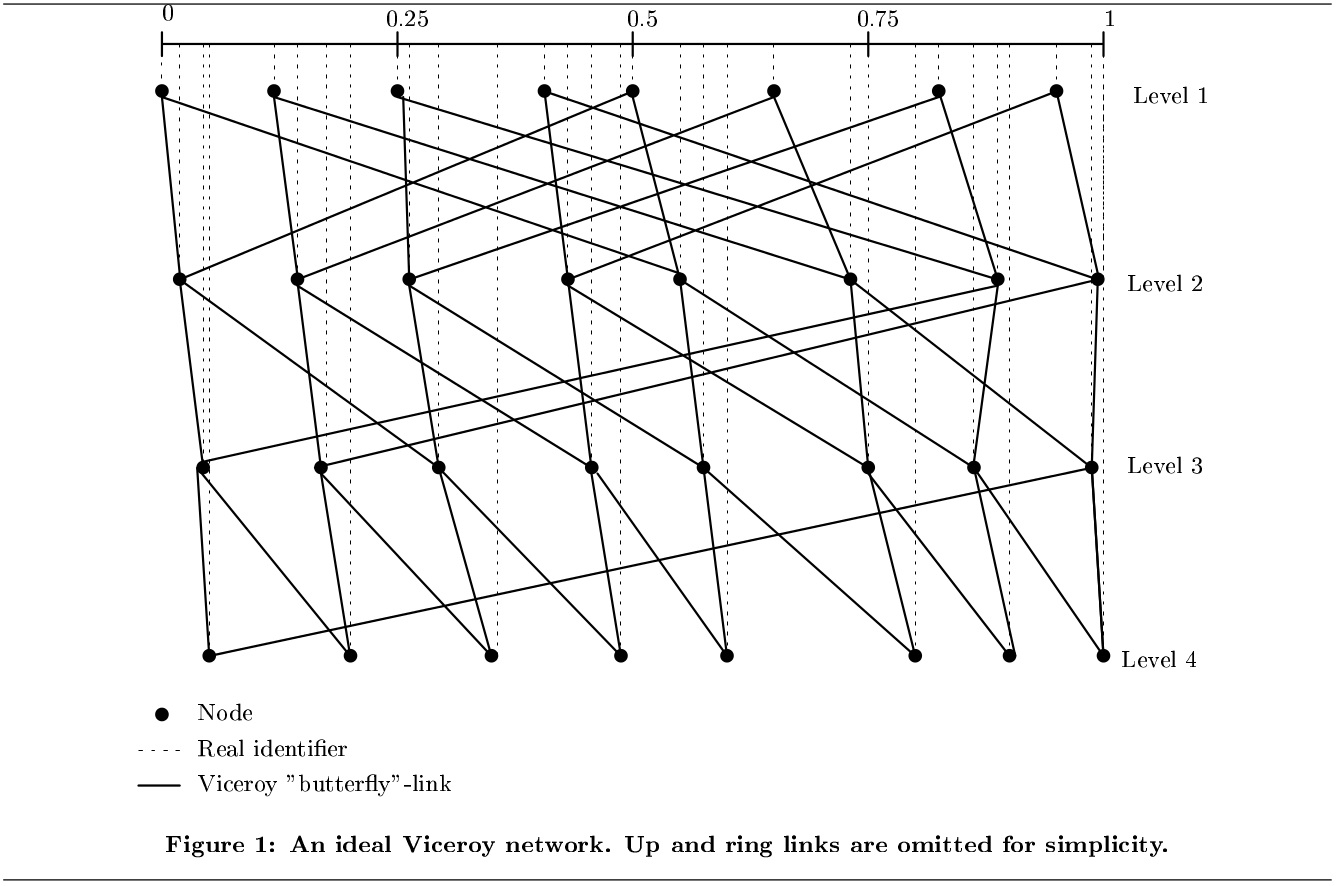
\includegraphics[width=1.0\textwidth]{viceroy}
\end{figure}


\section{Kelips}










\chapter{Small World Networks}
\section{The Small World}


Milgram and his fellow scientists performed a short series of experiments to study and quantify this phenomenon \cite{milgram1967small}.  
Subjects in these experiments were to route a postal message to a target person; for example the wife of a Cambridge divinity student in one experiment and a Boston stockbroker in another \cite{milgram1967small}.
The messages were only to be routed by forwarding them to a friend they thought most likely to know the target.

In the experiment with the target Boston stockbroker \cite{travers1969experimental}, 296 subjects from Nebraska were chosen as starting points.
Of the 64 messages that successfully made their way to the destination, the average path length from a subject to a participant was only 5 hops.  
People separated by great distances were nevertheless connected by short sequence of connections.

Researchers began to ask the question: if this experiment can get a message across the US, how can we model this behavior mathematically and use it for computer messages?


\subsection{Algorithmic View}


\cite{watts1998collective} 


Kleinberg examined a 2x2 lattice grid rather than a ring, which was examined in previous experiments by Watts and Strogatz  \cite{watts1998collective}
 (This is fine, rings are 1x1 grids)

%From Kleinberg paper
%Although we have focused on the two-dimensional grid, our analysis can be applied more
%broadly. We can generalize our results to k-dimensional lattice networks, as well as slightly
%“irregular” lattices; in the k-dimensional case, a decentralized algorithm can construct paths
%of length polynomial in logn if and only if r = k. Our results suggest a general model for

\cite{kleinberg2000navigation}
\cite{kleinberg2000small}


What happens when things aren't uniform?
\section{Symphony}

(this section is being done from memory at the moment)
Symphony closely resembles Chord, in that both use a 1-d ring structure and that the improvements made in here can be applied to Chord

Addressing:  Rather than using a keyspace of 0 to $2^n - 1$, Symphony assigns node on point between 0 and 1.  This is arbitrary (although it gets me thinking, is there any advantage/statistical properties   that could be exploited by making the space monic).

Peerlist:  (Besides a successor and predecessor list) Symphony maintains a list of $f$ fingers, randomly distributed according to the function defined in Kleinberg's small world routing.  This yields an average lookup of $O((log^{2} n)/f)$.  Note that when $f$ is log(n), Symphony's degree and lookup time is the same as most other DHTs.  

Peerlist maintenance is much simpler than Chord's.  Each finger is pinged periodically.  When a finger fails to respond, a new finger is chosen probabilistically .  The disadvantage is that there is no guarantee of a minimum routing time.

Security:  As the peerlist is chosen at random

Routing  is the same as Chord, for the most part, except for the 1-ahead lookup (below)



Proposed/implemented improvements not independent to Symphony
Bidirectional routing
1-ahead lookup - The node retrieves the peerlist of all it's peers and uses that in routing decisions.  While more expensive, there is a significant reduction in latency (not sure if a mathematically demonstrated amount, but it is experimentally demonstrated).  Using this could expose a network to an Eclipse attack.


\chapter{Outliers}
\section{Omniscient Routing}





\section{Geographic Hashing}
Under certain circumstances, it is sometimes more beneficial to store data according to the data's ``name,'' rather than being stored at the point where it was gathered.
This approach is data-centric storage or DCS.
The Geographic Hash Table (GHT) 
\cite{ratnasamy2002ght} was a system created to meet the demands of DCS, namely a scalable system that is resilient in the face of node failures and changes to the topology.  
It must also be able to take in to account energy resources.
The context assumes that nodes know their location via GPS or some other mechanism, that only a small number of access points connect the network to the outside, and energy is an essential resource that needs to be managed.


The central feature of GHT is the hashing of a key to a geographic location.  
The node responsible for the key's location (and the thus the key) is called the \textit{home node}.  
It is built atop the GSPR \cite{karp2000gpsr} routing system, which is a greedy, position-based routing scheme and exploits their characteristics

\subsection*{GPSR}
Greedy Perimeter Stateless Routing (GPSR) \cite{karp2000gpsr} uses a greedy approach to find a path from the source to the destination.
Upon obtaining the physical location of the destination \footnote{GPSR assumes that some given server is available to all nodes in the network. This location server would be able to provide the physical location all nodes in the network. It would only need to be communicated with once at the start of each connection.}, the node will forward it to the neighbor closest to the destination. 
That neighbor will in turn forward the message to his neighbor closest to the destination.
This continues until the destination receives the message.
Once a connection is successfully established, each the two endpoints append their location to each packet to keep each other informed of their positions.

Due to the nature of greedy forwarding, the protocol need a way to deal with the problem of a local maximum. 
In other words, the node has to have another option if it is the closest to the destination among the set of it and its neighbors.
The perimeter part of the name comes from how GPSR deals with this situation.
When some node is the local maximum, it will use the right hand rule to select a neighbor in an attempt to ``circle around'' the gap separating the node from the destination\footnote{A failure of GSPR is that it doesn't take velocity into account.}.
GHT exploits this this failsafe perimeter routing.  

\subsection*{GHT}
Data is stored in the home node, the node closest to the geographic destination.
GHT does not explicitly spell out how a node determines the home node, but under GPSR nodes should know the location of all the neighboring nodes in their perimeter.  
%fault tolerence
Data is replicated at nodes around the home node.  This is done using the perimeter routing mode in GSPR.
The \textit{Perimeter Refresh Protocol} means nodes check for network changes each defined period of time and update the replicas and home node as network changes dictate.





\section{Voronoi Based Schemes}




\subsection{RayNet}

Beaumont et al argues that a loose structure enough for searching.  Assume a $d$-dimension space, each dimension tied to some attribute of an object and each object identified by a unique set of values.  Objects should be linked to other objects that are close in the space.


\section{Sloppy Hashing}

Okay!  My misunderstanding was that this isn't a DHT.  It's a service the runs on top of a DHT (Chord, as it turns out).  But it gets really interesting.

Claims
The underlying point is  that many nodes in the network should have local copies of a popular file, but the DHT won't direct traffic to these copies, just the  (which  might be handled by a replica, unbeknownst to the person doing the lookup.
Storing data on the DHT (see CFS) is wasteful.
The last hops of a lookup are the ones that can be least optimized (can we fix that?  The reason is that lg n lookup time works by reducing the search space by half each hop.  The last few are over a very small space.  Would it help optimize routing in any way if an equal amount was covered at each hop?  Instincts say no, but I don't think it's been explored conclusively)
Concepts
Nodes are members of multiple DSHTs of differing diameters. 
Rather than each key being associated with one value, a key has multiple values (values typically being addresses that can be used to access the file associated with the key).  Rather than storing the data, metadata about file access is stored.  This actually seems like a good idea
Metadata of some kind (access info) is what is stored on the DSHT, not data.
Insertion works like normal until the max values are reached, in which  case we backtrack (somehow) and insert there (with a timestamp).
Get(key) traverses the overlay like normal.  Once a node holding values for the sought key is found.  Those values, as previously noted, are addresses for actually obtaining the file. 
The spillover helps with load balancing and eliminate (or mitigate hot spots)
Still have to deal with the issue of latency.  Create a hierarchical lookup layer.
Instead of a single system, multiple DSHTs exist at different levels.
Nodes are members of one  DSHT at each level (default 3), using the same nodeid in each.
Insertion inserts the key value on all three levels 
Getting looks locally first, then expands outwards.  The scheme has a guarantee that it will not take longer than a lookup on a  global table, but initial lookups are fast  (is this really different than a regular DHT, though?)
Clusters have two conflicting goals
Clusters should be large, so files can be found
Clusters should have a small diameter. for better latency.







\chapter{MANETS}
%Or who's idea was it that the darn things don't actually move!
One of the key features that make a DHT ideally suited for MANETs is the WYZYG nature of the network.  When you create an overlay on computers over the Internet, each hop on the overlay is actually multiple hops on the ``underlay''.  This is never the case on MANETs.

\chapter{Computing on A DHT}

\section{Features that lend to Distributed Computing}
\subsection{Metadata reduction}
\subsection{Decentralization}
\subsection{Caching and Replication}
\subsection{Fault Tolerance}

\section{MapReduce With DHTs}
\subsection{ChordReduce}

\section{ZHT}
The world is small because here, you know everyone.

Summary: ZHT\cite{li2013zht} uses O(n) degree to achieve O(1) hops.   It gets aways with this because it's intended for deployment in an isolated environment, so churn and updating the routing tables essentially  become a non-issue. It should be taken seriously because it has been successfully implemented.

ZHT is a DHT specifically designed for high-end computing.  The paper initially discusses  some areas of difficulty in scaling parallel deployments.  The two big issues are 1)  separating the storage and computation over a network cannot scale from peta to exa.  2) Basic metadata operations must scale.  Google's GFS and Yahoo's HDFS both use a centralized metadata manager that performs worse than other options.

As ZHT is specifically designed for a massively parallel deployment, certain constraints normally necessary for DHT operation are relaxed.  ZHT assumes that it is deployed on a network that is fast, trusted, and churn happens at a much much lower degree.  The latter two have the most significant impact to design.

 As the network can safely be assumed to be trusted, security is handed off to the local firewalls and network details.   The assumption is that an adversary should not be able to interact with the DHT at all.  

The largest design factor is that there is no significant churn to speak of.  In general, all the nodes start up when the network starts and shutdown when the network shuts down.  This  allows the process of building the routing tables to be done all as part of network boot (in effect, it now doesn't matter how long it takes to build them now, or what the overhead is, because that's just part of "booting").  It also implies that the routing tables will rarely change.  

These features let each node in ZHT hold a routing table with an entry with each other node in the network, which would incur much greater and overwhelming level of overhead in any  other typical deployment.  Implementation demonstrated that the memory cost was 32 bytes per entry in the node's routing table and they achieved a goal of < 1$\%$ memory footprint.

ZHT does work with dynamic networks, where nodes join and leave (at much lower rates than normal,  joining controlled by the network admin, leaving will typically only happen because of hardware failure or maintenance).  Joins and departures  are handled by migrating partitions, contiguous portions of keyspace, but partitioning is only discussed in abstract terms.

The other notable feature of DHT is its append operation, which allows stored data  to be concurrently modified.  ZHT has been thoroughly tested using  supercomputers and large clusters and the paper is more of a discussion of implementation. 


\section{Volunteer Computing With DHTs}
\section{Grid Based Computing with DHTs}
\bibliography{notes}
\bibliographystyle{ieeetr}

\end{document}
